
%%%%%%%%%%%%%%%%%%%%%%%%%%%%%%%%%%%%%%%%%%%%%%%%%%%%%%%%%%%%%%%%%%%%%%%%%%%%%%%
%%%%%%%%%%%%%%%%%%%%%%%%%%%%%%%%%%%%%%%%%%%%%%%%%%%%%%%%%%%%%%%%%%%%%%%%%%%%%%%
%%%%%%%%%%%%%%%%%%%%%%%%%%%%%%%%%%%%%%%%%%%%%%%%%%%%%%%%%%%%%%%%%%%%%%%%%%%%%%%
\section{Results} %-----------------------------------------------------------%
\subsection{Evaluation Platform} %--------------------------------------------%
All results were obtained by either interrogating
(Figure~\ref{probe_json}) the daemon directly or by running queries
against the SOSflow databases, such as the one in
Figure~\ref{example_query}.
%
\begin{figure}[h]
  \centering
  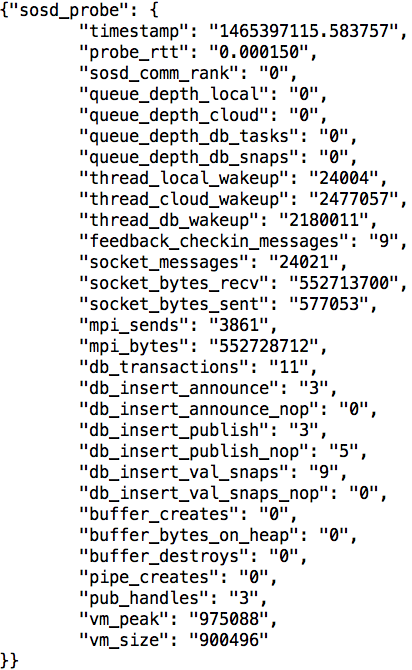
\includegraphics[width=\columnwidth]{images/probe_json_example.png}
  \caption{JSON Object Returned by SOS's Probe Tool}
  \label{probe_json}
\end{figure}
%
%
%


\subsection{Experiment Setup} %-----------------------------------------------%
%
\subsubsection{Oregon:ACISS} %-------------------------------------------------------%
Tests run on the ACISS platform at the University of Oregon were
deployed with the Torque job scheduler as MPICH2 MPI applications at
scales ranging from 3 to 24 nodes, serving 10 configurable synthetic
data-producing processes per node in all cases.
%
The ACISS battery of runs were tuned as stress tests to make ensure
the daemons could operate under reasonably heavy loads.
%
In the 24-node ACISS experiment (Figure~\ref{aciss_lat_24_agg}),
SOSflow processed 72,000,000 values during a 90 second window
containing three rounds of extremely dense API calls.
%


\subsubsection{NERSC:Cori} %--------------------------------------------------%
Real-world use case experiments were conducted on the Cori
supercomputer at The National Energy Research Scientific Computing
Center NERSC.
%
An SOSflow-enabled variant of the Tuning and Analysis
Utilities program (TAUflow) was created as a part of the SOSflow
development work.
%
On Cori, TAUflow was used to instrument the Livermore Unstructured
Lagrangian Explicit Shock Hydrodynamics (LULESH) code.
%
During the execution of LULESH, a thread in TAUflow would periodically
awaken and submit all of TAU's observed performance metrics into the
SOSflow system.
%
Power and memory consumption data was collected and stored in SOSflow
for each node and process.
%%%%%


\subsubsection{LLNL: Catalyst} %----------------------------------------------%
Latency tests were performed on the Catalyst machine at LLNL using up
to 128 nodes with 8 data sources contributing concurrently on each
node.
%
The latency observed at the on-node database at all
scales was not significantly different.
%
Only the results from the largest 128-node runs are presented here, as
the ``time in flight'' queue latency at smaller scales linearly
approaches the on-node injection latency figures.
%
These tests measured the latency for a cross-product of three
different parameters :
\begin{itemize}
\item Count of unique values per publication handle
\item Number of publish operations per loop
\item Delay between calls to the publish API
\end{itemize}

\subsubsection{Aggregation Topology}
%%%%%
In the presented version, SOSflow is configured at launch with a set
number of aggregator databases.
%
The validation tests on ACISS used 3 sosd(db) instances to divide up
the workload, while the TAUflow + LULESH experiments on Cori used a
single aggregator.
%
The parameter sweep runs on the LLNL Catalyst machine were done with
four aggregation sosd(db) targets.
%
The ACISS and Catalyst runs both featured dedicated nodes for the
aggregation databases because they were primarily designed to profile
the latency of data movement through SOSflow, so it was important
for the aggregator to not be contending with other on-node work.
%
The Cori run captured a real application's behavior, and was primarily
intended to demonstrate the fitness of SOSflow for capturing the
performance of a scientific workflow with meaningful context, so the
consistency of the aggregator's performance was less significant.
%
As many instances of aggregators can be spawned as needed in order to
support the quantity of data being injected from a global
perspective.
%
Because all data is tagged with a GUID, sharded aggregate databases
can be concatenated after the run concludes without collision of
identities wiping out unique references.
%%%%%




\subsubsection{Latency} %-----------------------------------------------------%
When a value is published from a client into the SOSflow runtime,
it enters an asynchronous queue scheme for both database injection
and off-node transport to an aggregation target.
%
Latency in this context refers to the amount of time that a value
spends in these queues before becoming available for query by
analytics modules.
%
\par
%
Values were being injected into the SOSflow system faster than
they could be spooled from the queues into the database.  This accounts
for the observed saw-tooth pattern of increasing latency.
%
While every value will eventually be processed and injected into the data
store, some values wound up having to wait longer than others as the queue
depth increased.
%
The asynchronous queues have thread-sequential FIFO ordering, but
because the MPI messages are queued up based on their arrival time,
and a batch is handled competely before the next is processed, there
is no real-time interleaving of database value injections, they are
injected in batches.
%
This creates the sawtooth pattern in figures~\ref{aciss_lat_3_agg} and
\ref{aciss_lat_24_agg}, as the latency for values in the batches near
the bottom of the pile of MPI messages consistently increases until
their batch is injected, detailed in
figure~\ref{aciss_lat_3_agg_detail}.
%%%%%

%%%%%
\begin{figure}[!t]
\centering
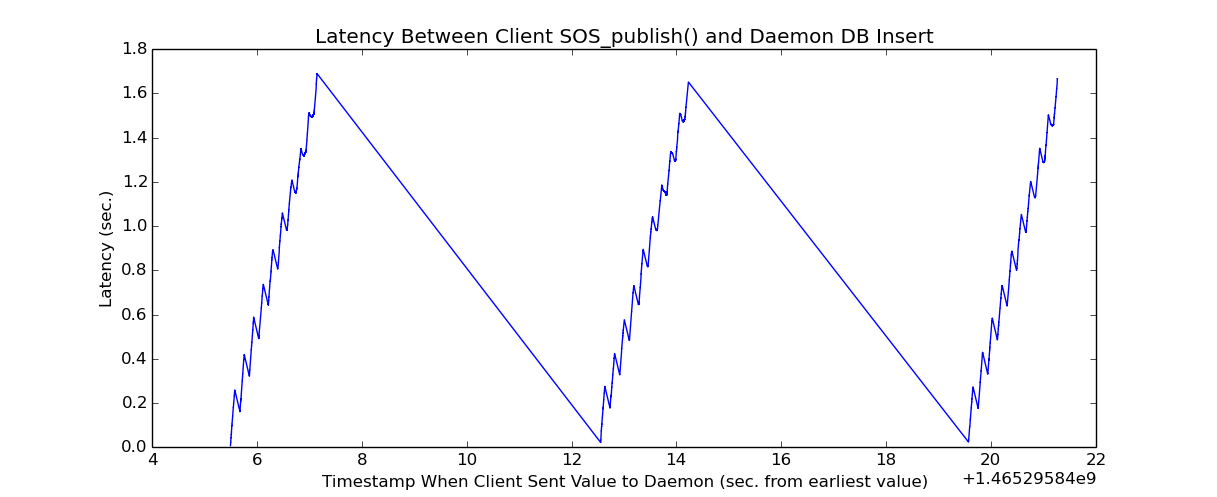
\includegraphics[width=\columnwidth]{images/aciss_latency_3_situ.png}
\caption{In Situ Latency (3 Nodes, 30 Applications)}
\label{aciss_lat_3_situ}
\end{figure}
%%%%%

%%%%%
\begin{figure}[!t]
\centering
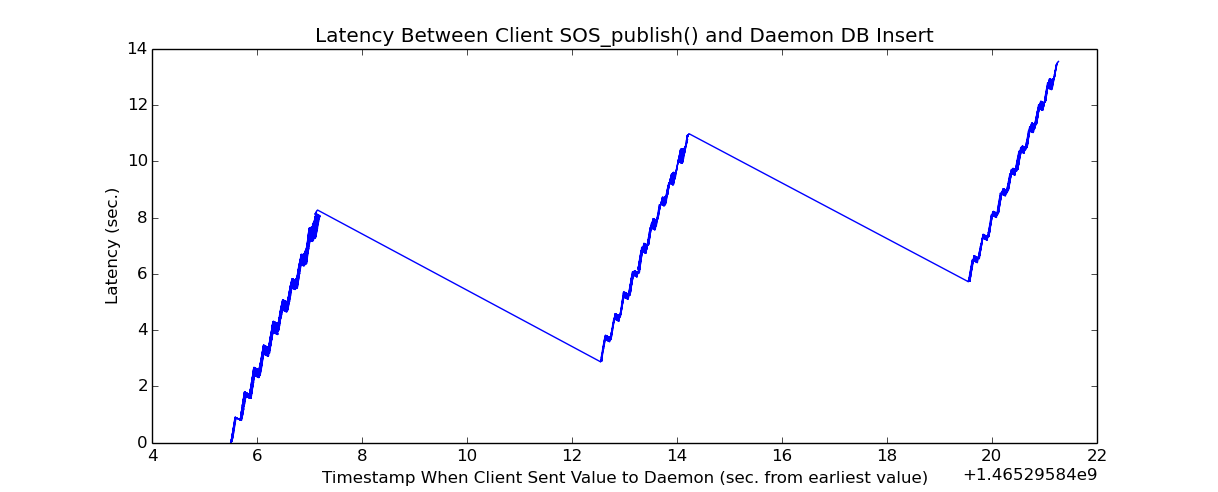
\includegraphics[width=\columnwidth]{images/aciss_latency_3_agg.png}
\caption{Aggregate sosd(db) Latency (3 Nodes, 30 Applications)}
\label{aciss_lat_3_agg}
\end{figure}
%%%%%

%%%%%
\begin{figure}[!t]
\centering
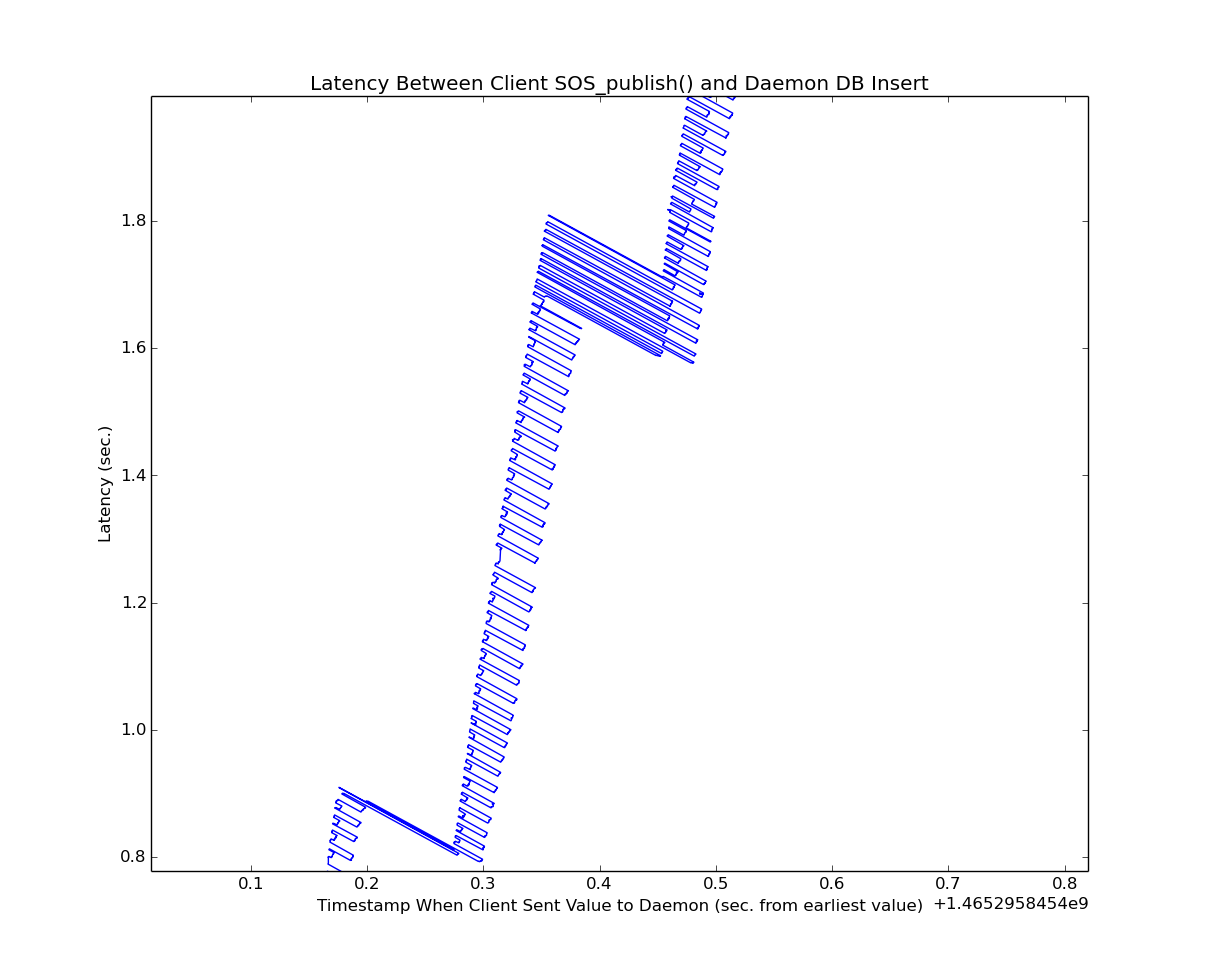
\includegraphics[width=\columnwidth]{images/aciss_latency_3_agg_zm.png}
\caption{Aggregate sosd(db) Detail (3 Nodes, 30 Applications)}
\label{aciss_lat_3_agg_detail}
\end{figure}
%%%%%

%%%%%
\begin{figure}[!t]
\centering
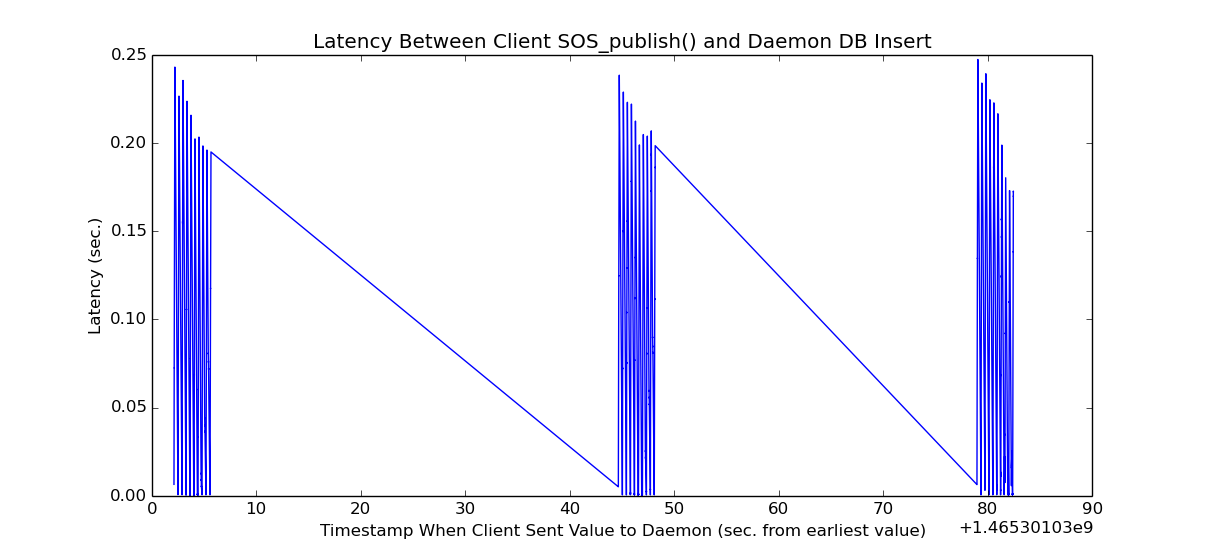
\includegraphics[width=\columnwidth]{images/aciss_latency_24_situ.png}
\caption{In Situ Latency (24 Nodes, 240 Applications)}
\label{aciss_lat_24_situ}
\end{figure}
%%%%%

%%%%%
\begin{figure}[!t]
\centering
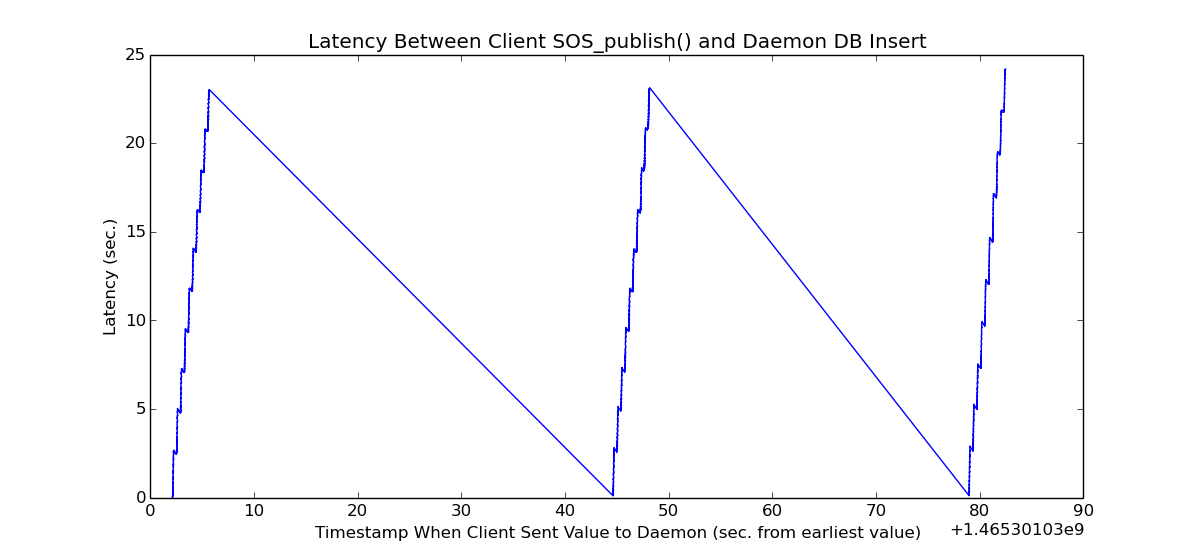
\includegraphics[width=\columnwidth]{images/aciss_latency_24_agg.png}
\caption{Aggregate sosd(db) Latency (24 Nodes, 240 Applications)}
\label{aciss_lat_24_agg}
\end{figure}
%%%%%
%
\par
%



\subsubsection{Time Cost of Publish API Call} %-------------------------------%
In situ interactions with the daemon are nearly constant time
operations regardless of the daemon's workload.
%
This is shown in figures~\ref{sock_cost} and \ref{sock_cost_detail},
where the round trip time (RTT) of a probe message between a client
and the daemon (blue) is projected over a graph of the number of new
messages arriving in a sample window (red).
%
\par
%
This information was fetched by sending 9000+ probe messages over a 15
minute window, with a single sosd(listener) rank processing an average
of 43,423 client messages a minute arriving from four different
processes on an 8-way Xeon node.
%
The messages from SOS clients contained more than 14.7 GB of data,
averaging to 338kB per message.
%
Though there are a few spikes in the probe message RTT visible in
Figure~\ref{sock_cost}, they are likely not related to SOSflow at all,
as Figure~\ref{sock_cost_detail} reveals in detail.
%
The RTT holds steady during low and high volume of traffic from the
other in situ client processes.
%
The mean RTT for the probe messages was 0.003 seconds, and the maximum
RTT was 0.007 seconds.
%%%%%
\begin{figure}[h]
\centering
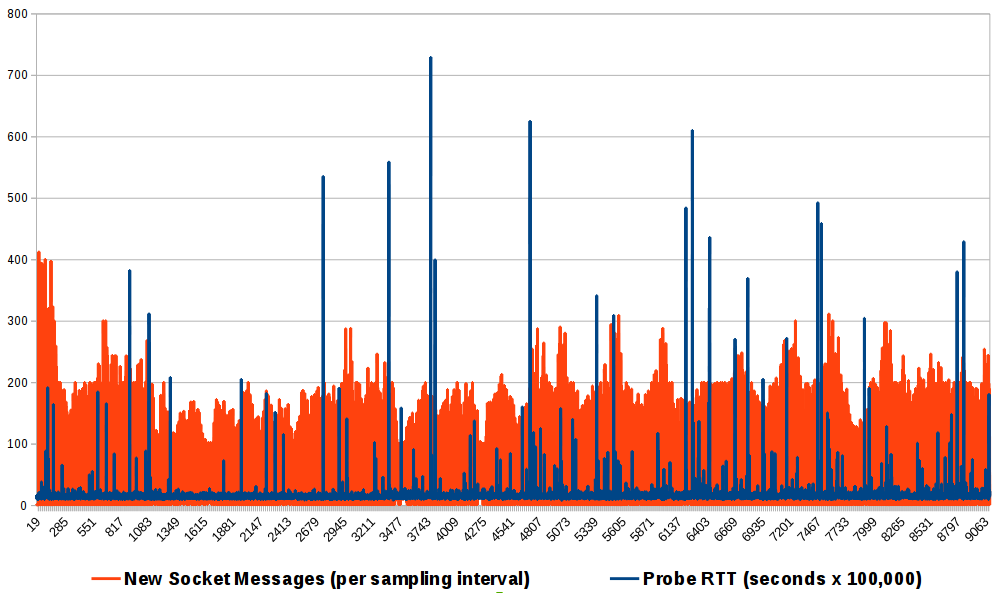
\includegraphics[width=\columnwidth]{images/icebox_api_cost_when_slam.png}
\caption{SOSflow Socket Communication Cost (~0.003sec Mean)}
\label{sock_cost}
\end{figure}
%%%%%

%%%%%
\begin{figure}[h]
\centering
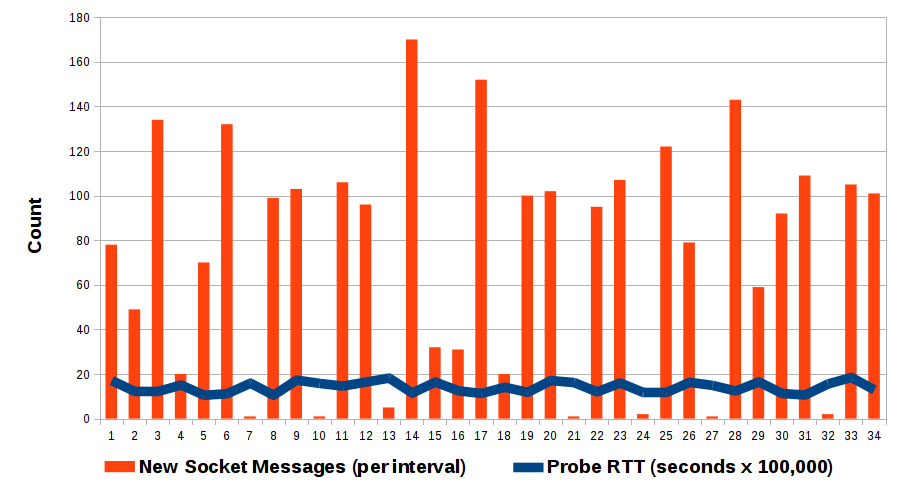
\includegraphics[width=\columnwidth]{images/icebox_api_cost_zoom.png}
\caption{SOSflow Socket Communication Cost, Detail}
\label{sock_cost_detail}
\end{figure}
%%%%%
%
\par
%
These results are promising, because they represent a worst-case
scenario for API calls: Unlike the SOSflow API calls for publishing
data, the probe message is relatively slow, as the daemon has to
immediately service the request by packaging up a struct of its
internal statistics to send back.
%



\subsection{Discussion} %-----------------------------------------------------%
%
Many of the behavioral characteristics of SOSflow are the product of
its internal parameters and the configuration of its runtime
deployment, rather than products of its data model and algorithms.
%
The exploration of optimal settings in that combined parameter space
is left for future work: For now the effort was made to select
reasonable default SOSflow configuration parameters and
typical/non-priviledged cluster queues and topologies.
%
Because of the general novelty of the architecture, the results
presented here could be considered the \textit{performance baseline}
for SOSflow to improve on as the research line matures.




%%%
%%%  EOF
%%%
